
%%%%%%%%%%%%%%%%%%%%%%%%%%%%%%%%%%%%%%%%%%%%%%%%%%%%%%%%%%%%%%%%%%%%%%%%%%%%%%
%%% Preamble

%%% Document Type
\documentclass[11pt,openany]{memoir} % 'openany': allows chapters to open on left and right pages; avoids blank pages between chapters to force opening on right
\chapterstyle{section}

%%% Packages
\usepackage{amsmath,amssymb,cancel,units} % math environment and symbols
\usepackage{array}                        % for better arrays (eg matrices) in maths
\usepackage{paralist}                     % very flexible & customisable lists (eg. enumerate/itemize, etc.)
\usepackage{verbatim}                     % adds environment for commenting out blocks of text & for better verbatim
\usepackage[pdftex,bookmarks,colorlinks,breaklinks]{hyperref}  % PDF hyperlinks, with coloured links
\usepackage{memhfixc}                     % remove conflict between the memoir class & hyperref
\usepackage{graphicx}                     % Add graphics capabilities
\usepackage{xspace}                        % smart space insertion after commands
\usepackage{tabulary}
\usepackage[table]{xcolor} % http://tex.stackexchange.com/questions/5363/how-to-create-alternating-rows-in-a-table
\usepackage{wrapfig}
\usepackage{xspace}

%% Following allows for bulleted definition lists ('description' environment)
%% by declaring \SpecialItem before the list;
%% from: http://tex.stackexchange.com/questions/57876/add-bullet-points-to-description-lists
\let\Item\item
\newcommand\SpecialItem{\renewcommand\item[1][]{\Item[\textbullet~\bfseries##1]}}
\renewcommand\enddescription{\endlist\global\let\item\Item}


\usepackage{listings}
\definecolor{mygreen}{rgb}{0,0.6,0}
\definecolor{mygray}{rgb}{0.5,0.5,0.5}
\definecolor{mymauve}{rgb}{0.58,0,0.82}

\lstset{ %
  backgroundcolor=\color{white},            % choose the background color; you must add \usepackage{color} or \usepackage{xcolor}
  basicstyle=\footnotesize\ttfamily,        % the size of the fonts that are used for the code
  breakatwhitespace=false,                  % sets if automatic breaks should only happen at whitespace
  breaklines=true,                          % sets automatic line breaking
  captionpos=b,                             % sets the caption-position to bottom
  commentstyle=\color{mygreen},             % comment style
  deletekeywords={...},                     % if you want to delete keywords from the given language
  escapeinside={\%*}{*)},                   % if you want to add LaTeX within your code
  extendedchars=true,                       % lets you use non-ASCII characters; for 8-bits encodings only, does not work with UTF-8
  frame=single,	                            % adds a frame around the code
  columns=fullflexible,
  keepspaces=true,                          % keeps spaces in text, useful for keeping indentation of code (possibly needs columns=flexible)
  keywordstyle=\color{blue},                % keyword style
  % language=Octave,                          % the language of the code
  otherkeywords={*,...},                    % if you want to add more keywords to the set
  % numbers=left,                             % where to put the line-numbers; possible values are (none, left, right)
  % numbersep=5pt,                            % how far the line-numbers are from the code
  % numberstyle=\tiny\color{mygray},        % the style that is used for the line-numbers
  rulecolor=\color{black},                  % if not set, the frame-color may be changed on line-breaks within not-black text (e.g. comments (green here))
  showspaces=false,                         % show spaces everywhere adding particular underscores; it overrides 'showstringspaces'
  showstringspaces=false,                   % underline spaces within strings only
  showtabs=false,                           % show tabs within strings adding particular underscores
  stepnumber=2,                             % the step between two line-numbers. If it's 1, each line will be numbered
  stringstyle=\color{mymauve},              % string literal style
  tabsize=2,	                            % sets default tabsize to 2 spaces
  title=\lstname                            % show the filename of files included with \lstinputlisting; also try caption instead of title
}

%%% Notation and Variables

\newcommand{\archipelagoModel}{\textit{Archipelago}\xspace}
\newcommand{\archipelagoPackage}{\texttt{archipelago}\xspace}
\newcommand{\targetData}{D}
\newcommand{\trainingDataForModel}[1]{D^{*#1}}
\newcommand{\trainingDataSet}{\mathbf{D}^{*}}
\newcommand{\summaryStatisticFunction}{S}
\newcommand{\modelCategory}[1]{M_{#1}}
\newcommand{\modelCategories}{\mathbf{M}}

%%%%%%%%%%%%%%%%%%%%%%%%%%%%%%%%%%%%%%%%%%%%%%%%%%%%%%%%%%%%%%%%%%%%%%%%%%%%%%%
%% Main Document
\begin{document}
% \rowcolors{2}{gray!25}{gray!15}

\title{ARCHIPELAGO}
\author{Jeet Sukumaran}
\maketitle
\setsecnumdepth{subsubsection}

\tableofcontents

\chapter{Introduction}

``\archipelagoModel'' is the name of a generative phylogeny-based model that simultaneously incorporates the diversification processes of speciation and extinction nad the biogeographical processes of area gain (``dispersal'') and area loss (``extirpation''), with these processes being differentially regulated by ecological or other traits that are themselves co-evolving on the phylogeny.
The theory and background to this model and its usage is described in the following paper:


This software project, \archipelagoPackage, presents a suite of programs to generate and analyze data under the \archipelagoModel model.
The primary objective of the analysis is \textit{model selection}: i.e., statistically identifying the model that generated a particular set of data.
% to \textit{classify a dataset with respect to the model that generated it}.
The suite of programs constituting \archipelagoPackage is, thus, a computational biogeographical model selection analysis package that exploits the power and flexibility of the \archipelagoModel model to allow you to ask and answer historical biogeographical questions of a nature and complexity that are not possible under any other approach.
In particular, instead of asking questions about ancestral area patterns, you can ask questions about processes, and how some processes (e.g., ecology) affect other processes (e.g., dispersal or speciation).

\chapter{Installation}

\section{Pre-requisites}

\begin{itemize}
    \item Python 2.7 or higher
    \item DendroPy Phylogenetic Computing Library, version 4 or above (\url{http://dendropy.org}).
    \item R (\url{http://www.r-project.org/})
    \item The following R packages:
    \begin{itemize}
        \item adegenet
        \item picante
        \item BioGeoBears
        \item GEIGER
    \end{itemize}
\end{itemize}

\section{Installation from Source}

Run the following in the top-level directory of the project:

\begin{lstlisting}
    python setup.py install
\end{lstlisting}


\chapter{Usage}

\section{Overview of Workflow}

\begin{figure}[h!]
    \begin{center}
        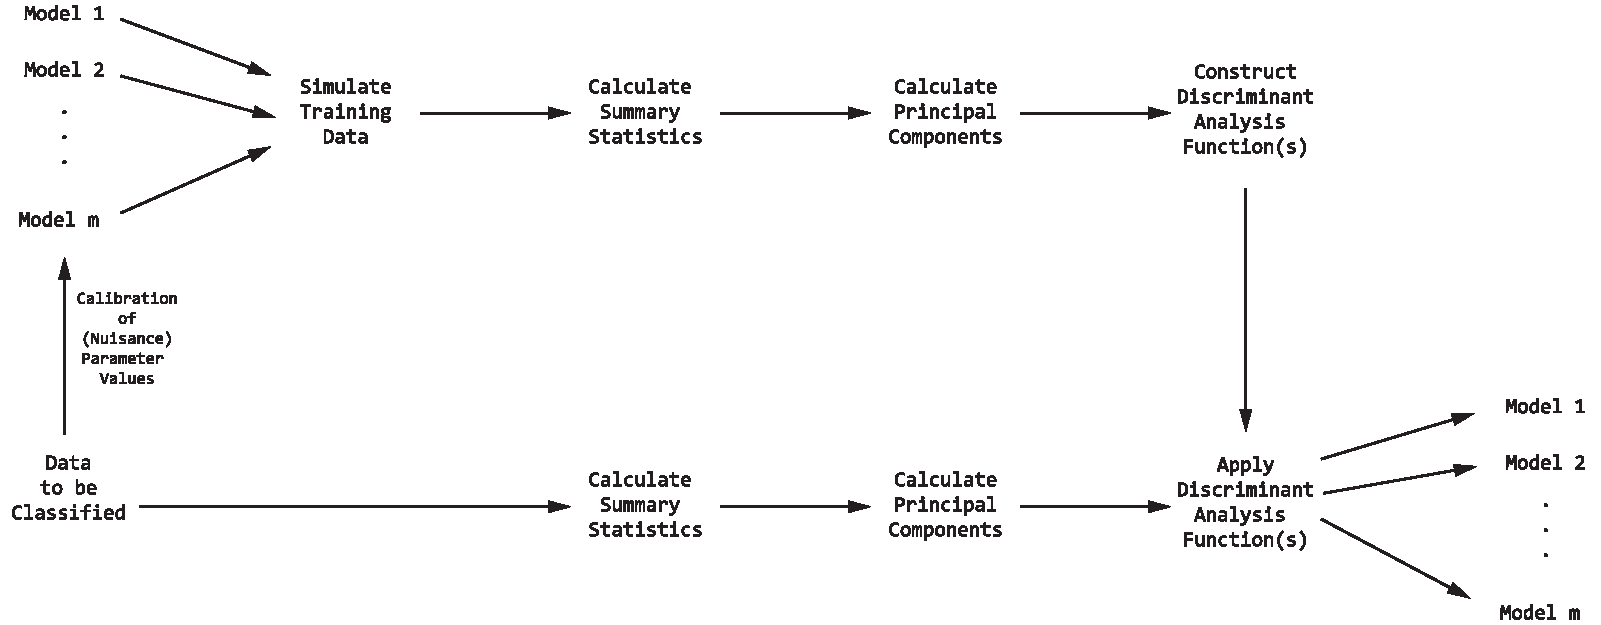
\includegraphics[scale=0.5]{figs/flowchart1.pdf}
        % \caption{default}
        % \label{fig:default}
    \end{center}
\end{figure}

Let $\targetData$ be the \textit{target} data, consisting of an ultrametric phylogeny with each of the tips associated with a geographic range (presence/absence over one or more areas) as well as with set of trait states.
Let $\modelCategories = \{\modelCategory{1}, \modelCategory{2}, ... \modelCategory{m}\}$ be a set of $k$ models that we are interested in studying.
Let $\summaryStatisticFunction(\cdot)$ be a function that takes a set of data returns a set of summary statistics.
Our analytical objective is, for each $\modelCategory{i}, \modelCategory{i} \in \modelCategories$, estimate the probability that it generated the target data $\targetData$, relative to all the other models in $\modelCategories$.
The operational procedure consists of the following steps:
\begin{enumerate}
    \item \textbf{Simulation of Training Data}: For each $\modelCategory{i}, \modelCategory{i} \in \modelCategories$, simulate $n$ replicates of data, $\trainingDataForModel{i}$. We label each replicate of this data with the name of the model that generated it (e.g., ``Model $i$''). The set of all data so generated constitutes the training data, $\trainingDataSet$.
    \item \textbf{Calculation of Summary Statistics}: Calculate summary statistics on the training data to yield, $\summaryStatisticFunction(\trainingDataSet)$, and summary statistics on the target data to yield $\summaryStatisticFunction(\targetData)$.
    \item \textbf{Classification of Target Data}: Construct a Discriminant Analysis (DA) function on principal components (PC) calculated on the training data set summary statistics, $\summaryStatisticFunction(\trainingDataSet)$; apply the discriminant analysis function to principal components calculated on the summary statistics of the target data, $\summaryStatisticFunction(\targetData)$.
\end{enumerate}

\section{Simulation of Training Data}

We use the program, ``\texttt{archipelago-simulate.py}'', to simulate the data under each model in the set of competing models.
The simulation program is run separately for each of the models, with multiple independent replicates in each run.
Full details on this program invocation can be found by running:
\begin{lstlisting}
    archipelago-simulate.py --help
\end{lstlisting}
A typical invocation of the program will have the following arguments:
\begin{description}
    \SpecialItem
    \item[``MODEL-FILE''] \hfill \\
        A JSON or Python file containing nothing but a dictionary specifying the full model under which to simulate data. This is described in detail in the \hyperref[sec:workflow-model-specification]{Model Specification} section.
    \item[``\texttt{-n}'' or ``\texttt{--nreps}''] \hfill \\
        The number of independent replicates to simulate under this model.
    \item[``\texttt{-o}'' or ``\texttt{--output-prefix}''] \hfill \\
        The path and filename stem where the results will be saved.
\end{description}
For example,
\begin{lstlisting}
    archipelago-simulate.py -n 100 -o results/m1 model1.json
\end{lstlisting}
will run 100 replicates under the model specified in the file ``model1.json'' and all output will saved to files in the ``results/'' subdirectory with filenames beginning with ``m1''.

The simulation program produces the following output:
\begin{description}
    \label{sec:description-of-output-files}
    \SpecialItem
        \item[\texttt{<OUTPUT-PREFIX>.focal-areas.trees}] \hfill \\
            A collection of phylogenies in NEWICK format, where each phylogeny represents the result from a single simulation replicate.
            The tips of these trees represent lineages that occur in at least one of the focal areas (in contrast to the phylogenies in the ``\texttt{all-areas.trees}'' file, where \textit{all} extant lineages are represented, regardless of where they occur).
            The distribution and trait states of the tip lineages are encoded in the tip labels.
            This is the data that is of primary analytical interest, and will be passed to the summary statistics calculation program, \texttt{archipelago-summarize.py}.
        \item[\texttt{<OUTPUT-PREFIX>.all-areas.trees}] \hfill \\
            A collection of phylogenies in NEWICK format, where each phylogeny represents the result from a single simulation replicate.
            The tips of these trees represent \textit{all} extant lineages at the end of the simulation, regardless of whether or they occur in the focal areas.
            The distribution and trait states of the tip lineages are encoded in the tip labels.
        \item[\texttt{<OUTPUT-PREFIX>.log}] \hfill \\
            A detailed log of the run.
        \item[\texttt{<OUTPUT-PREFIX>.model.json}] \hfill \\
            A description of the model that the run executed. This can be used to confirm that the model used corresponded to the model that was input. In addition, for default settings or values may have been used aspects or parameters that were not specified in the input model file, and these are recorded here.
\end{description}


\subsection{Model Specification}
\label{sec:workflow-model-specification}
We specify the model under which we simulate data using \texttt{archipelago-simulate.py} by a \textit{model file}.
This is a JSON file providing a single dictionary as its only element.
An example of a basic model specification is:
% \lstinputlisting[language=Python]{source_filename.py}
\lstinputlisting{includes/samplemodel1.json}
The model dictionary consists of the following elements:
\begin{description}

    \item[``model\_id'']  \hfill \\
        This key takes an arbitrary string value that identifies the category or class of model being run.
        It will serve as the identifier of all data generated under this model.
        Each tree generated under this model will have the metadata item, ``\texttt{model\_id}'', with this value associated with it.
        Each set of summary statistics calculated on each tree will have an additional field, ``\texttt{model\_id}`` added to it to document the generating model by the value given to this field.
        The classification programn ``\texttt{archipelago-classify.py}'', will expect the training data summary statistics to have a column with this name, and it will use the values of this column to determine the origin or source of the data.
    \item[``areas'']  \hfill \\
        This key defines the geographical template.
        Its corresponding value is a list of dictionaries with the following keys, with each dictionary defining a distinct area:
        \begin{description}
            \item[``label'':] \hfill \\
                A unique \textbf{string} value giving the name or identifier for the area.
            \item[``is\_supplemental'':] \hfill \\
                A \textbf{boolean} (\texttt{true} or \texttt{false}) specifying whether or not the area is a focal area or a supplemental area.
                Focal areas are areas from which the lineages are sampled, while supplemental areas are area that interact with the focal areas ecologically, evolutionarily, and biogeographically, but are not sampled in the target data.
                For example, when analyzing a group of Western Pacific islands, we may consider the island groups to be focal areas, but Australia and Papua New Guinea may be considered supplemental areas, because our target data only spans lineages that have representatives in the focal areas, though there is no doubt that the evolutionary history of those lineages includes Australia and Papua New Guinea.
            \item[``area\_connection\_weights'':] \hfill \\
                A list of positive real values which provides the dispersal weights from the area being defined to all other areas, specified in the order when they are defined.
                Note that this includes the connection weight to the same area as well, and this is \textit{must} be set to $0.0$.
                If not specified, by default it is assumed that all areas are equally connected (i.e., connection weights default to $1.0$, except for the self-connection weight, which is $0.0$.).
        \end{description}

    \item[``traits'']  \hfill \\
        This key defines the traits.
        Its corresponding value is a list of dictionaries with the following keys, with each dictionary defining a distinct trait:
        \begin{description}
            \item[``label'':] \hfill \\
                A unique \textbf{string} value giving the name or identifier for the trait.
            \item[``nstates'':] \hfill \\
                A \textbf{non-zero positive integer} specifying the number of distinct states that the trait has.
            \item[``transition\_rate'':] \hfill \\
                A \textbf{positive real} specifying the mean rate of change per unit time for the trait.
            \item[``transition\_weights'':] (optional) \hfill \\
                A list of lists specifying the relative weights (as \textbf{positive real} values) for each state transition. If not given, equal rates are assumed for all transitions.
        \end{description}

    \item[``diversification'']  \hfill \\
        This key defines the diversification processes (speciation and extinction).
        It consists of a dictionary with the following two keys:
        \begin{description}
            \item[``lineage\_birth\_rate'':] \hfill \\
                A \textit{lineage-specific rate function definition} (see below) specifying the speciation rate.
            \item[``lineage\_death\_rate'':] \hfill \\
                A \textit{lineage-specific rate function definition} (see below) specifying the global extinction rate (i.e., the death rate in a birth-death branching process submodel, \textit{not} the ``extinction'' or area loss rate of the DEC biogeographical submodel).
        \end{description}

    \item[``anagenetic\_range\_evolution'']  \hfill \\
        This key defines the anagenetic range evolution processes (area gain and area loss).
        It consists of a dictionary with the following two keys:
        \begin{description}
            \item[``lineage\_area\_gain\_weight'':] \hfill \\
                A \textit{lineage-specific rate function definition} (see below) specifying the rate at which a lineage loses an area in its range.
                When set to a fixed value, this corresponds to the area gain rate in the BayArea model or the $d$ or ``dispersal'' parameter in the DEC model.
            \item[``lineage\_area\_loss\_rate'':] \hfill \\
                A \textit{lineage-specific rate function definition} (see below) specifying the rate at which a lineage loses an area in its range.
                When set to a fixed value, this corresponds to the area loss rate in the BayArea model or the $e$ or ``extinction'' (really, ``extirpation'') parameter in the DEC model.
        \end{description}

    \item[``cladogenetic\_range\_evolution'']  \hfill \\
        This key defines the relative weights of the cladogenetic range evolution speciation modes.
        It consists of a dictionary with the following keys, with the value of each key being the weight of that mode relative to all other modes:
        \begin{description}
            \item[``sympatric\_subset\_speciation\_weight'':] \hfill \\
                Default value: $1.0$.
            \item[``single\_area\_vicariance\_speciation\_weight'':] \hfill \\
                Default value: $1.0$.
            \item[``widespread\_vicariance\_speciation\_weight'':] \hfill \\
                Default value: $1.0$.
            \item[``founder\_event\_speciation\_weight'':] \hfill \\
                Default value: $0.0$.
        \end{description}

    \item[``termination\_conditions'']  \hfill \\
        This key defines the conditions which determine when the simulation should end.
        Its value is a dictionary consisting of \textit{one} of the following keys:
        \begin{description}
            \item[``target\_focal\_area\_lineages'':] \hfill \\
                A non-zero positive integer that specifies the minimum number of extant lineages that occur across all focal areas.
                Once this number is reached or exceeded, the simulation terminates.
                Typically, if this mode of termination is used, this will be set to the number of tips of the target data phylogeny.
            \item[``max\_time'':] \hfill \\
                A positive real number that specifies the maximum time the simulation should run.
                Typically, if this mode of termination is used, this will be set to the root age of the target data phylogeny.
        \end{description}

\end{description}

\subsection{Lineage-Specific Rate Function}

A number of process rates (speciation, extinction, area gain, area loss) are specified in terms of a ``lineage-specific rate function''.
This allows the rate of the process to vary depending on the trait state or other attributes of the lineage.
For each process, the rate function can be specified in one of four ways: a fixed value, a (Python) lambda expression, a trait state mapping, or as a Python function object.

\subsubsection{Fixed-Value Lineage-Specific Rate Function}
With a fixed-value lineage-specific rate function, the rate of the process is the same, fixed, constant value regardless of lineage.
That is, all lineages unconditionally have the same rate for the process throughout their lifetimes in the simulation.
A fixed-value lineage-specific rate function is specified by providing a dictionary like the following as the value for the process key:
\begin{lstlisting}
{
    "definition_type": "fixed_value",
    "definition": 0.01,
}
\end{lstlisting}
The actual value of the ``definition'' entry would, of course, vary depending on the model.
Typically, if not of analytical interest, this would be estimated based on the target data.
Fixing the rate of a process to a value estimated from the target data is known as ``calibrating'' the model.
More sophisticated approaches can be used to take into account uncertainty in the rate estimates.
For example, sets of simulations can be run under different values of the process rate sampled from a prior.

\subsubsection{Trait State Mapping Lineage-Specific Rate Function}
\label{sec:trait-state-mapping}
Here, you provide a list of rate values for that processes parameter, with a one-to-one correspondence to the states of an trait defined previously.
For example, if you have defined a trait with the label ``color'' and three states:
\begin{lstlisting}
{"label": "color", "nstates": 3, "transition_rate": 0.01}
\end{lstlisting}
you could define a process that takes on the rate of $0.0$ if the ``color'' trait of a lineage was in state $0$, $0.5$ if the trait was in state $1$, and $1.0$, if the trait was in state $2$ by specifying:
\begin{lstlisting}
{
    "definition_type": "trait_state_index_map:color",
    "definition": [0.0, 0.5, 1.0],
}
\end{lstlisting}

\subsubsection{Lambda-Expression Rate Function}
The rate function is given as a Python lambda function definition.
The lambda function should take a single argument, an object of the ``Lineage'' class, and return a real value representing the rate of the process for this particular lineage at this particular point in time.
For example, the following replicates the above trait state mapping:
\begin{lstlisting}
{
    "definition_type": "lambda_definition",
    "definition": "lambda lineage: 0.0 if lineage.traits_vector[0] == '0' else (0.5 if lineage.traits_vector[0] == '1' else 1.0)"
}
\end{lstlisting}
Note that trait \textit{types} are 0-based numeric indexes, while trait states are character values, ``0'', ``1'', ``2``, etc. \archipelagoPackage internally uses character values to specify trait states as this allows for special states such as ``NA'' or ``null''.

As another example, the following inspects the distribution vector of a lineage and returns a rate of $1.0$ if the first area is occupied and $0.5$ if not:
\begin{lstlisting}
{
    "definition_type": "lambda_definition",
    "definition": "lambda lineage: 1.0 if lineage.distribution[0] == 1 else 0.5"
}
\end{lstlisting}
In constrast to trait states, absence/presence in an (0-based indexed) area is indicated by \textit{numeric} values, $0$ and $1$, respectievly.
% \begin{description}
%     \item[``definition\_type'':] \hfill \\
%         The type of function. The value associated with this key is one of the following string values, which communicates the type of function that is being defined:
%         \begin{itemize}
%             \item ``fixed\_value''
%             \item ``lambda\_definition''
%             \item ``trait\_state\_index\_map:TRAIT-LABEL''
%             \item ``function\_object''
%         \end{itemize}
%     \item[``definition'':] \hfill \\
%         The actual definition. The format and content of the value depends on the the ``\texttt{definition\_type}'', and is described below.
%     \item[``description'':] \hfill \\
%         The value of this is a string providing a description oft the rate
% \end{description}
% \begin{description}
%     \item[``definition\_type'':] \hfill \\
%         The type of function. The value associated with this key is one of the following string values:
%         \begin{description}
%             \item[``fixed\_value'':] if the definition for the function is a specified as fixed, real value. In this case, the rate of the process is considered invariant with respect to the lineage.
%             \item[``lambda\_definition'':] if the definition for the function is given as a string value providing a (Python) lambda expression.
%                 The lambda function should take a single argument, an object of the ``Lineage'' class, and return a real value representing the rate of the process for this particular lineage at this particular point in time.
%             \item[``trait\_state\_index\_map:TRAIT-LABEL'':] if the definition for the rates is given as a list of values that are indexed by the state of the trait previously defined with the label, ``\verb+<TRAIT-LABEL>+''. The list should contain one value for every state of the trait. For example, given a trait defined as:
% \begin{lstlisting}
% {"label": "color", "nstates": 3, "transition_rate": 0.01}
% \end{lstlisting}
%             \item[``function\_object'':] if the definition for the function is a function object.
%                 Note that this cannot be defined in a JSON file or in a Python file passed as input to the ``archipelago-simulate.py'' program.
%                 For this option, the simulations need to be run using a dedicated user script that calls the library simulation routines directly.
%                 While more complex than the ``archipelago-simulate.py'' program, this option provides the maximum flexibility and power in specifying the model, as it allows for an arbitrarily complex Python function, making use of user-defined classes and functions, as well as both standard and third-party libraries/packages.
%         \end{description}

% \subsection{``Calibrating'' the Models}

% The \archipelagoModel model has a number of processes that require rates to be specified, including:

% \begin{itemize}
%     \item The birth rate
%     \item Trait evolution rates
%     \item The (global) rate of area gain
%     \item The (global) rate of area loss
% \end{itemize}

% In some cases, these rates are naturally specified as part of the various competing hypotheses being tested.
% In others, they are nuisance parameters that are not an integral part of the hypotheses being tested.
% The simplest way to specifying these rates is to estimate them from the target data.
% For example, the birth rate can be estimated using from an existing phylogeny using DendroPy or a number of R packages, such as GEIGER.
% The trait evolution rates can be estimated (separately for each trait) using BayesTraits or the R package, GEIGER.
% The rate of area gain and loss can be estimated using lagrange, BioGeoBears, BayArea, or RevBayes.

\section{Calculation of Summary Statistics}
\label{sec:workflow-calculation-of-summary-statistics}

\section{Classification of Target Data}
\label{sec:workflow-classification-of-target-data}

\section{Profiling the Target Data}
\label{sec:workflow-profiling-the-target-data}

\section{Encoding the Target Data}
\label{sec:workflow-encoding-the-target-data}

To \hyperref[sec:workflow-calculation-of-summary-statistics]{calculate the summary statistics} or \hyperref[sec:workflow-profiling-the-target-data]{profile the target data} using \archipelagoPackage, we need to communicate the trait and geographical data associated with the tips of the the target phylogeny to the program.
This is achieved by encoding the information in the labels of the phylogeny.
The tip label for each lineage consists of \textit{three} components separated by a carat (``\verb+^+'') character:

\begin{lstlisting}
s68^1.2.0^0011
\end{lstlisting}

The first component (``s68'' in the above example) is an arbitrary species index that uniquely identifies each lineage.

The second component (``1.2.0'' in the above example) is the vector of trait states for the species.
The states of each trait for the lineage is represented by an integer index separated by a period.
In this example, there are three trait types, with the value of the first trait type ``1'', the second ``2'', and the third ``0''.
Note that the first trait state is indexed by 0, not 1.
That is, if there are ``n'' states, then the set of valid trait state indexes is $\{0, 1, 2, ..., n-1\}$.
All lineages in the system must have the same number of trait types (three, in this example), and the trait state values are assumed to be given in sequential order.

The third component (``0011'' in the above example) is the geographical presence/absence vector for the lineage, where ``0'' indicates the absence of a lineage from the area, and ``1'' indicates the presence.
In this example, the lineage is absent from the first and second areas, but present in the third and fourth. All lineages must have their presences or absences specified in all areas.

Consider a system given by the following phylogeny:
\begin{lstlisting}
[&R] ((A:1,B:1):3,(C:3,(D:2,E:2):1):1);
\end{lstlisting}
where the traits are represented by the following character matrix:
\begin{lstlisting}
    A   001
    B   011
    C   201
    D   100
    E   211
\end{lstlisting}
and the distribution over six areas is represented by the following incidence matrix:
\begin{lstlisting}
    A   110001
    B   010011
    C   101101
    D   001100
    E   011111
\end{lstlisting}
We would then encode this information in the phylogeny as follows:
\begin{lstlisting}
    [&R] ((A^0.0.1^110001:1,B^0.1.1^010011:1):3,(C^2.0.1^101101:3,(D^1.0.0^001100:2,E^2.1.1^011111:2):1):1);
\end{lstlisting}

\chapter{Walk-Through of a Basic Analysis}

\begin{wrapfigure}{r}{0.6\textwidth}
% \begin{figure}[h!]
  \vspace{-20pt}
    \begin{center}
        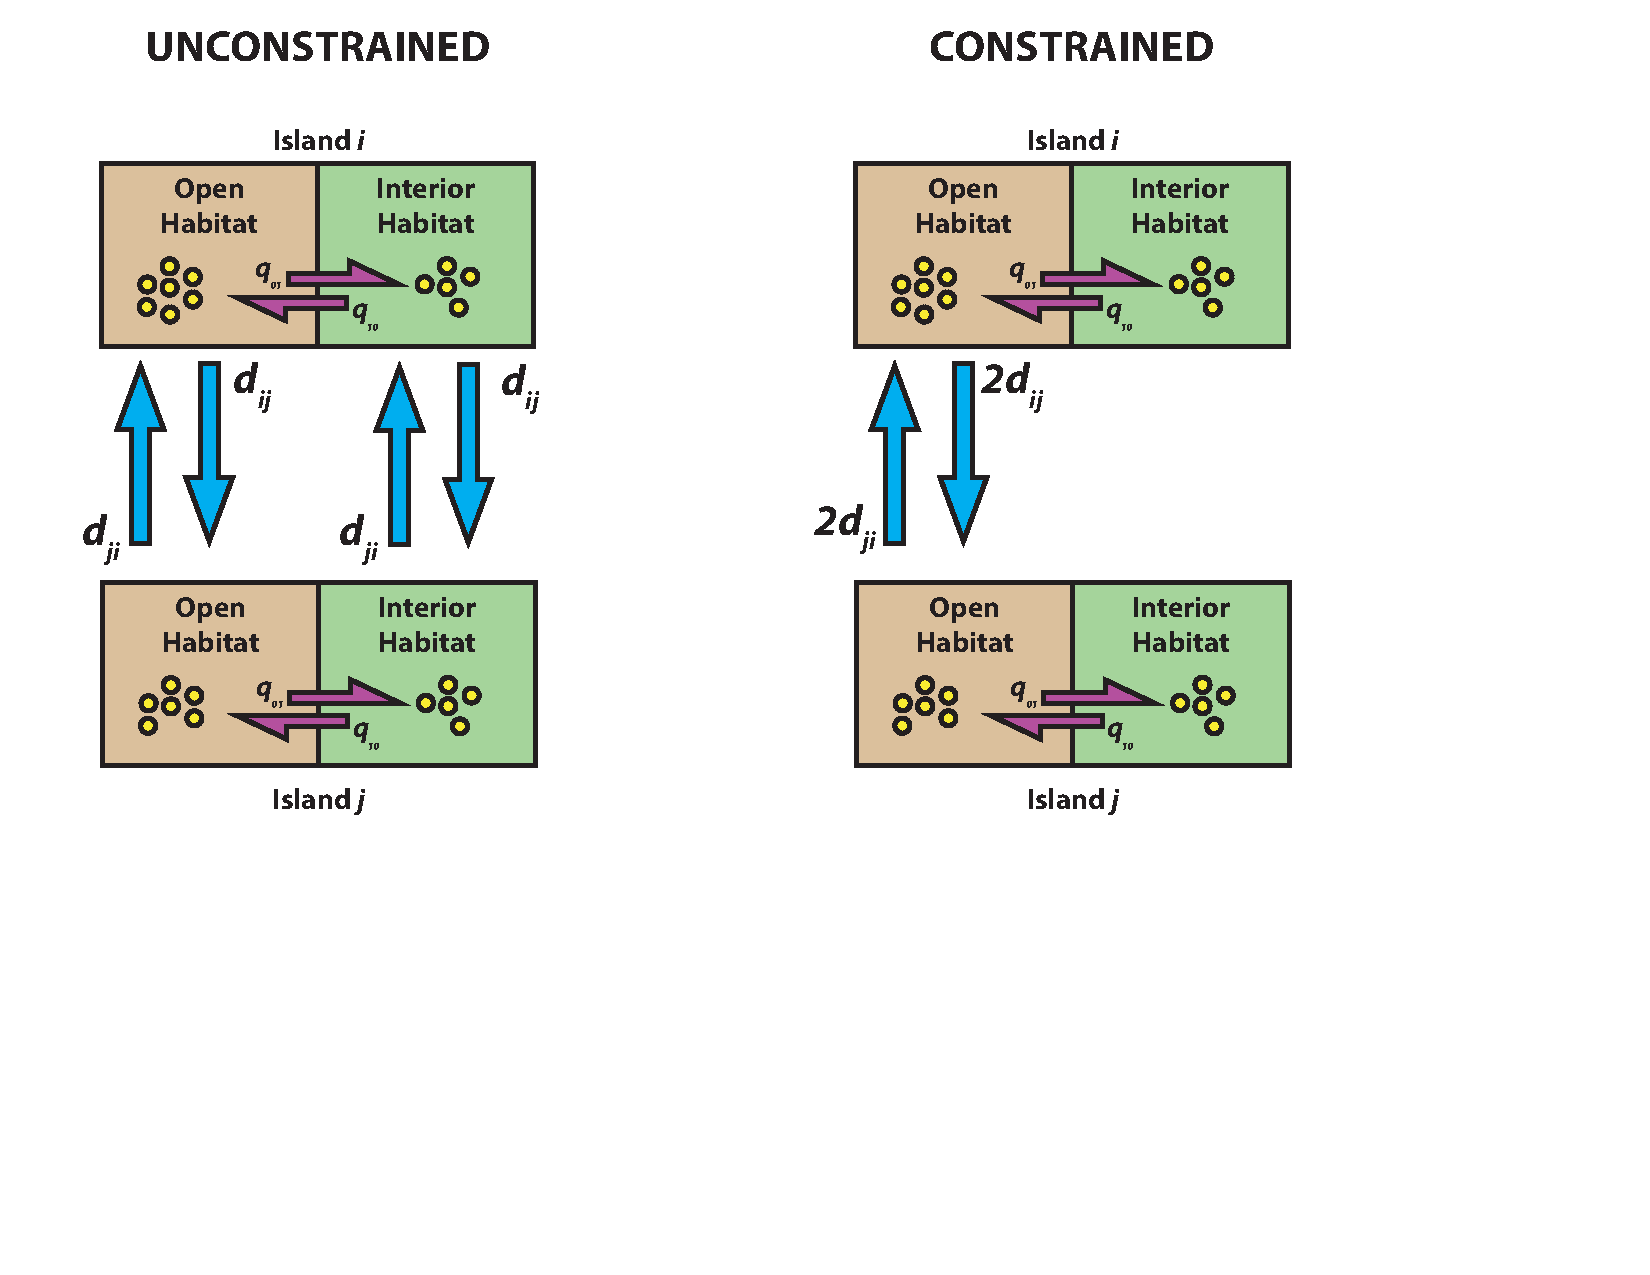
\includegraphics[scale=0.30]{figs/Experimental-Design-1.pdf}
        % \caption{default}
        % \label{fig:default}
    \end{center}
  \vspace{-80pt}
% \end{figure}
\end{wrapfigure}

\section{Analytical Objectives}

As an example of a very basic analysis, let us consider testing whether or not dispersal is constrained by habitat association of a lineage (Figure).
We propose two different models, each corresponding to a different dispersal regime.
In the ``unconstrained'' model, lineages are free to disperse between islands regardless of their habitat affinities.
In the ``constrained'' model, ony lineages associated with the disturbed or open habitats can disperse between islands, while lineages associated with interior habitats are not able to disperse.
The habitat affinities of the lineages themselves are modeled as a discrete binary trait that evolves stochasitcally over the phylogeny.
That is, each lineage has a habitat trait, which can either be in the ``disturbed'' or ``interior'' state, and the state of this trait determines whether or not the lineage is capable of dispersing in the ``constrained'' model.
Thus, in the unconstrained model, lineages disperse between interior habitats on different islands directly.
In the constrained model, on the other hand, lineages cannot disperse between interior habitats directly: they have to move into a disturbed habitat association in ecological space over evolutionary time, at which phase they are capable of dispersing into new islands, and then re-invade the interior habitats on those new islands by, again, moving into them in ecological space over evolutionary time.

\section{The Target Data}

We will analyze the data set discussed in Sukumaran \textit{et al.} 2015.
This is a data set of birds in Wallacea, originally presented in Carstensen \textit{et al.} 2013.
We will be focussing on a subset of 365 species for which sufficient ecological data is available that allows us to categorize them into either ``open'' (disturbed) or ``undisturbed'' habitat species.
The data, model files, etc. for this analysis can be found in the ``\texttt{examples/wallacea\_bird\_dispersal\_by\_habitat/}'' subdirectory of the project directory.
The subdirectory ``\texttt{original-data}'' has the full phylogeny of 549 species (``\texttt{master\_tree.nexus}''), from the Jetz \textit{et al.} (????) paper as well as a comma-separated value formatted file with the geographical, ecological, and other information from the Carstensen \textit{et al.} 2013 paper.

\section{Simulating the Training Data}

We will simulate data under two classes of models: ``unconstrained'' and ``constrained''.
In this analysis, we will be using the basic DEC biogeography model as our bigeography (sub)model.
We will need to specify the following rates:

\begin{itemize}
    % \item[The cladogenesis (speciation or birth) rate] \hfill \\
    %     In the DEC model as implemented by largrange and BioGeoBEARS, speciation is not an explicit process: the model is conditioned on the speciation event timings and structure given by the input phylogeny, which is (typically) taken as truth.
    %     However, in \archipelagoModel, we explicitly model the diversification process and sample phylogenies as part of the training data.
    %     While \archipelagoModel supports a full birth-death model, we will not be modeling lineage extinction directly under this model.
    %     Instead, following the DEC model, we will model lineage extinction as part of
    % \item[The (global) rate of area gain]
    %     ...
    % \item[The (global) rate of area loss]
    \item The speciation or birth rate \hfill \\
        \\
        In the DEC model as implemented by largrange and BioGeoBEARS, speciation is not an explicit process: the model is conditioned on the speciation event timings and structure given by the input phylogeny, which is (typically) taken as truth.
        However, in \archipelagoModel, we explicitly model the diversification process and sample phylogenies as part of the training data.
        While \archipelagoModel supports a full birth-death model, we will not be modeling lineage extinction directly under this model.
        Instead, following the DEC model, we will model lineage extinction as part of the biogeographical submodel, with a lineage going extinct when its range is reduced to the null set, i.e. when it has lost all areas from its range.
        The speciation process is a nuisance process with respect to our study question, and both ``unconstrained'' and ``constrained'' classes of models will be set to the same fixed speciation rates.
        We will estimate the speciation rate under a pure-birth Yule model using the empirical target phylogeny.
    \item The trait transition rate \hfill \\
        \\
        We use a simple equal-rates (ER) trait transition submodel.
        As with the diversification submodel, the trait evolution process is nuisance process with respect to our study question, and both ``unconstrained'' and ``constrained'' classes of models will be set to the same fixed trait transition rate, as estimated from the empirical target data.
    \item The global rate of area gain \hfill \\
        \\
        This corresponds to the ``dispersal'' or ``$d$'' parameter in the DEC model.
        We will estimate this rate based on the empirical target data under the basic DEC model, using lagrange, BioGeoBEARS, BayArea, or RevBayes.
        In the ``unconstrained'' class of model, this rate will be used unmodified.
        In the ``constrained'' class of model, we will use a trait-state mapping function which will return a rate of $0$ if the lineage habitat trait is in ``interior'' state and \textit{twice} the global dispersal rate estimated if the lineage trait is ``disturbed'' state.
        We use twice the rate so that the total dispersal flux across the system is maintained, given that, under an equal-rates traits model, we expect half the lineages to be in ``interior'' habitat state and consequently only half the lineages (the ones in the ``disturbed'' habitat state) to be actively dispersing.
    \item The global rate of area loss \hfill \\
        \\
        This corresponds to the ``extinction'' (extirpation) or ``$e$'' parameter in the DEC model.
        We will estimate this rate based on the empirical target data under the basic DEC model, using lagrange, BioGeoBEARS, BayArea, or RevBayes.
        The rate of area loss is the same under both the ``unconstrained'' and ``constrained'' models, and thus the estimated rate will be used as a fixed rate for this process under both these models.

\end{itemize}

\subsection{Estimating the Rate Parameters from the Empirical Data to Calibrate the Simulations}

Setting the parameters for the various processes (diversification, area gain, area loss, etc.) is known as \textit{calibrating} the model.
As noted above, this is typically done by setting the rates to estimates based on the target data.
The \archipelagoPackage package provides a program, ``\texttt{archipelago-profile.py}'' that conveniently does this for you.
It requires that the target phylogeny labels have \hyperref[sec:workflow-encoding-the-target-data]{trait and geographical data encoded}.
The subdirectory ``\texttt{target-data}'' of the Wallacean example directory has the original phylogeny pruned down to the 365 species that are the focus of this study, with \hyperref[sec:workflow-encoding-the-target-data]{trait and geographical data encoded in the labels}.
We can run the profiler program on this phylogeny to yield the training data process rate parameters:
\begin{lstlisting}
archipelago-profile.py --estimate-dec-lagrange target-data/wallacea.newick
\end{lstlisting}
if we have (the C++) \texttt{lagrange} installed, or, otherwise:
\begin{lstlisting}
archipelago-profile.py --estimate-dec-biogeobears target-data/wallacea.newick
\end{lstlisting}
if we want to estimate the DEC model parameters using \textit{BioGeoBEARS}.

This program will provide a ``profile'' of this phylogeny (provide MLE's of speciation, trait transition, area loss, and area gain rates).
The result is a comma-separated value (CSV) formatted-file with one entry per tree passed to it.
As here we are only using a single tree, there is only one data row.
The results can be seen in the file ``\texttt{wallacea.profile.csv}'' which includes the following information:


\begin{table}[htp]
\label{tbl:exampleProfile}
\begin{center}
\footnotesize
\begin{tabulary}{\linewidth}{ L L }
\hline \\ [-1.5ex] % for correct spacing between line and first row
Field   &   Value \\
\hline \\ [-1.5ex] % for correct spacing between line and first row
num.tips                        & 365 \\
root.age                        & 106.998428 \\
pure.birth.rate                 & 0.05482309568853121 \\
trait.1.est.transition.rate     & 0.062247 \\
area.est.transition.rate        & 2.396912 \\
biogeobears.dec.dispersal.rate  & 0.018156246 \\
biogeobears.dec.extinction.rate & 0.002645152 \\
\hline
\end{tabulary}
\end{center}
\end{table}%

\subsection{Setting up the Training Data Models}

We will create two models to generate the training data, ``unconstrained'' and ``constrained''.
The files corresponding to these models can be found in the ``\texttt{examples/wallacea\_bird\_dispersal\_by\_habitat/training-data-models}'' subdirectory of the project: ``\texttt{unconstrained.json}'' and ``\texttt{constrained.json}'', respectively.

The first entry in each model file is the identifier for each of the models:

\begin{minipage}[t]{0.475\textwidth}
\textbf{\texttt{unconstrained.json}:}
\begin{lstlisting}
{
"model_id": "unconstrained",
}\end{lstlisting}
\end{minipage}
\begin{minipage}[t]{0.475\textwidth}
\textbf{\texttt{constrained.json}:}
\begin{lstlisting}
{
"model_id": "constrained",
}\end{lstlisting}
\end{minipage}

These identifiers are crucial to allow the training data items to be assigned to the correct generating model, which itself is crucial for the proper construction of the discriminant analysis functions.
The model identifiers will be assigned to the each tree generated by the simulations under each model, and will be propagated through rest of the pipeline by other programs.

Both models share the same geographical template, consisting of four focal areas and two supplemental areas, and are coded identically.
The four focal areas represent the four island ``modules'' in the original data: Banda Sea, Lesser Sundas, Maluku, and Sulawesi.
The two supplemental areas represent the two continental sources: Sundaland (Asia) and the Sahul Shelf (Australia and Papua New Guinea).
\begin{lstlisting}
"areas": [
    { "is_supplemental": true, "label": "b1" },
    { "is_supplemental": true, "label": "b2" },
    { "is_supplemental": false, "label": "a1" },
    { "is_supplemental": false, "label": "a2" },
    { "is_supplemental": false, "label": "a3" },
    { "is_supplemental": false, "label": "a4" }
], \end{lstlisting}

Both models also share the same trait regime: a single two-state trait, representing the habitat associated with each lineage.
We use the trait transition rate estimated under an equal-rates model on the original data as the training data simulation trait transition rate.
\begin{lstlisting}
"traits": [
    { "label": habitat, "nstates": 2, "transition_rate": 0.062247}
],
\end{lstlisting}
Both models also share the same diversification regime, and we use the birth rate estimated from the original data as the fixed, constant birth rate for both models.
We also set the death rate to a fixed, constant rate of $0.0$ for both models.
(The Archipelago model distinguishes between the death rate of the birth-death branching process, which is sometimes referred to as the ``extinction'' rate, and the rate of area loss, which is also called the ``extinction'' rate in the original DEC model description and related literature.
Here, following the DEC model, we do not explicitly model extinction of lineages, but instead model extinction implicitly through modeling of the rate of area loss.)
\begin{lstlisting}
"diversification": {
    "lineage_birth_rate": {
        "definition_type": "fixed_value",
        "definition": 0.05486829846551938
    },
    "lineage_death_rate": {
        "definition_type": "fixed_value",
        "definition": 0.0
    }
},\end{lstlisting}

The anagenetic rate of area gain is where the models differ.
In the ``unconstrained'' model, the rate of area gain is a fixed, constant value, as estimated on the original data:
\begin{lstlisting}
"anagenetic_range_evolution": {
    "lineage_area_gain_rate": {
        "definition_type": "fixed_value",
        "definition": 0.018156246
    },
    .
    .
    .
\end{lstlisting}
However, in the ``constrained'' model, we only allow lineages that are associated with a state index of ``0'' (which we are arbitrarily assigning to mean the ``open'' or ``disturbed'' state) are allowed to disperse.
Lineages that are associated with a state index of ``1'' are restricted from dispersing.
We use a \hyperref[sec:trait-state-mapping]{trait state mapping} function to specify this regime.
Here, we identify the trait by the label that we assigned to it in the trait definition (``habitat'') in the ``definition\_type'' field, and for the ``definition'' field we provide a list of values, with each element in the list specifying the rate rate for the state with the corresponding index, so that the first rate is associated with the first trait state, the second rate is associated with the second trait state, and so on.
Note that we \textit{double} the estimated rate of area gain ($0.036312492 = 2 \times 0.018156246$).
This is because we want to maintain the same overall dispersal flux in the system as in the empirical data.
We used a factor of $2$ based on the fact that, for the equal-rates trait model we are assuming here, the equilibrium frequency of each state is $0.5$.
Thus, at equilibrium, only half the lineages will be in the dispersal state, $0$, which means that only half the lineages will be dispersing.
If we were to naively assign the estimated dispersal rate to the area gain rate, we would end up with half as much dispersal in the system as in the original data.
This can easily be verified by simulating data under this and then re-estimating the dispersal rates.
By assigning twice the estimated dispersal rate as the area gain rate, to account for the fact that only half the lineages are dispersing, we correctly achieve parity with the dispersal rate in the original data.
\begin{lstlisting}
"anagenetic_range_evolution": {
    "lineage_area_gain_rate": {
        "definition_type": "trait_state_index_map:habitat",
        "definition": [ 0.036312492, 0.0 ]
    },
    .
    .
    .
\end{lstlisting}

If an asymmetric rates trait transition model is used, we would have to calculate the dispersal flux at equilibrium and correct the area gain rate using the appropriate factor to compensate.
For example, if the asymetrical-rate trait transition matrix has the following value:
\begin{align*}
\begin{bmatrix}
    0         &  7.55786 \\
    30.403915 & 0        \\
\end{bmatrix}
\end{align*}
then the stationary frequency of the first and second states are $0.8009086$ and $0.1990914$, respectively.
This means that if we were the restrict dispersal only to the first state, we would only have approximately $0.80$ of the lineages dispersing, and thus the total dispersal flux would fall short of that estimated from the empirical data.
To compensate, we would have to increase the area gain rate by a factor of $\frac{1}{0.8009086}=1.248582$, for a total rate of $0.02266844$ instead of $0.018156246$.
This system would be specified by the following
\begin{lstlisting}
"traits": [
    { "label": habitat, "nstates": 2, "transition_rate": 1.0,
    "transition_weights":[[0,7.557866],[30.403915,0]]}
],
"anagenetic_range_evolution": {
    "lineage_area_gain_rate": {
        "definition_type": "trait_state_index_map:habitat",
        "definition": [ 0.036312492, 0.0 ]
    },
    .
    .
    .
\end{lstlisting}

For the area loss rate, again, both models are identical, and we use a fixed, constant value as estimated from the original data:
\begin{lstlisting}
"anagenetic_range_evolution": {
    .
    .
    .
    "lineage_area_loss_rate": {
        "definition_type": "fixed_value",
        "definition": 0.00257819
    }
}
\end{lstlisting}

Finally, we specify the duration for which to run each of the simulations.
We condition on the the number of tips in the original data, $365$, for both models:
\begin{lstlisting}
    "termination_conditions": {
        "target_focal_area_lineages": 365
    }
\end{lstlisting}

\subsubsection{Running the Simulations}
We use the program ``\texttt{archipelago-simulate.py}'' to simulate the training data.
We generate 200 replicates under each of the models, saving the results to appropriately named output locations:
\begin{lstlisting}
archipelago-simulate.py --nreps 200 --output-prefix unconstrained_training_data unconstrained.json
archipelago-simulate.py --nreps 200 --output-prefix constrained_training_data unconstrained.json
\end{lstlisting}
The above commands will generate two sets of output files, one beginning with the prefix ``unconstrained\_training\_data'' and the other beginning with the prefix ``constrained\_training\_data''.
See the \hyperref[sec:description-of-output-files]{output file description section} for details on the files produced.
Here, we are interested in the files with the extension ``\texttt{.focal-areas.trees}``: these are the phylogenies that we need for the next stage.
The above commands can be run on multiple computers simulataneously, or launched on the a multi-core computers multiple times in parallel, with all the ``\texttt{.focal-areas.trees}`` collected and passed to the next stage: summary statistic calculation.


\end{document}
